\documentclass[12pt,a4paper]{article}

% --- Essential Packages ---
\usepackage[utf8]{inputenc}
\usepackage{mathptmx} % Times New Roman font equivalent
\usepackage[top=0.8in, bottom=0.8in, left=1.0in, right=0.5in]{geometry}
\usepackage{setspace}
\usepackage{fancyhdr}
\usepackage{graphicx}
\usepackage{tikz}
\usepackage{eso-pic}
\usepackage{amsmath, amsfonts, amssymb}
\usepackage{algorithm}
\usepackage{tocloft}
\usepackage{algpseudocode}
\usepackage{booktabs}
\usepackage{cite}
\usepackage{titlesec}
\usepackage{caption}
\usepackage{url}
\usepackage{array}

% --- TikZ Libraries for High-Quality Workflow Diagram ---
\usetikzlibrary{shapes.geometric, arrows.meta, positioning, shadows, calc}

% --- Formatting Specifications ---
\setstretch{1.5}
\setlength{\parindent}{0.3in}
\setlength{\parskip}{4pt}

% Section Headings: 14pt Bold Left Aligned
\titleformat{\section}{\fontsize{14pt}{17pt}\bfseries\raggedright}{\thesection.}{0.5em}{}
\titleformat{\subsection}{\fontsize{12pt}{15pt}\bfseries\raggedright}{\thesubsection}{0.5em}{}

% Caption styling: Table titles at top, Figure titles below
\captionsetup[table]{position=top, font={small,bf}, skip=5pt}
\captionsetup[figure]{position=bottom, font={small,bf}, skip=5pt}

% Table of Contents dots and spacing
\renewcommand{\cftsecleader}{\cftdotfill{\cftdotsep}}

% --- Global Page Border (Single Line of width 3/4 pt = 0.75pt on Every Page) ---
\AddToShipoutPictureBG{%
    \begin{tikzpicture}[remember picture, overlay]
        \draw[line width=0.75pt]
            ([xshift=0.35in, yshift=-0.35in]current page.north west)
            rectangle
            ([xshift=-0.35in, yshift=0.35in]current page.south east);
    \end{tikzpicture}%
}

% --- Header/Footer Setup for Page Numbering ---
\pagestyle{fancy}
\fancyhf{}
\renewcommand{\headrulewidth}{0pt}
\cfoot{\thepage}

\begin{document}

% =========================================================================
% 1. TITLE PAGE (As per Department Format, No Page Number)
% =========================================================================
\begin{titlepage}
\thispagestyle{empty}
\begin{center}
    \vspace*{0.1in}
    {\fontsize{20pt}{24pt}\bfseries PEDESTRIAN CROWD HAZARD CLASSIFICATION AND DYNAMIC EVACUATION ROUTING SYSTEM \par}

    \vspace{0.25in}
    {\fontsize{14pt}{17pt}\bfseries PROJECT SYNOPSIS \par}
    \vspace{0.05in}
    {\fontsize{12pt}{15pt}\selectfont OF PROJECT-II (PROJ-IT781) \par}

    \vspace{0.25in}
    {\fontsize{14pt}{17pt}\bfseries BACHELOR OF TECHNOLOGY \par}
    \vspace{0.05in}
    {\fontsize{12pt}{15pt}\selectfont in \par}
    \vspace{0.05in}
    {\fontsize{16pt}{19pt}\bfseries Information Technology \par}

    {\fontsize{12pt}{15pt}\selectfont SUBMITTED BY \par}
    \vspace{0.12in}

    {\fontsize{12pt}{15pt}\selectfont
    \begin{tabular}{p{2.8in}p{2.8in}}
    \textbf{Aditya Paul} & \textbf{Univ. Roll No.:} 13000223009 \\
    \textbf{Ankita Biswas} & \textbf{Univ. Roll No.:} 13000223020 \\
    \textbf{Anushka Das} & \textbf{Univ. Roll No.:} 13000223023 \\
    \textbf{Archismita Maity} & \textbf{Univ. Roll No.:} 13000223024 \\
    \textbf{Bratik Mukherjee} & \textbf{Univ. Roll No.:} 13000223044 \\
    \end{tabular} \par}

    \vfill

    \vspace{0.15in}
    {\fontsize{12pt}{15pt}\selectfont Under the Supervision of \par}
    \vspace{0.05in}
    {\fontsize{14pt}{17pt}\bfseries PROF. (DR.) Bijoly Saha \par}
    \vspace{0.05in}

    \vspace{0.15in}
    
\includegraphics[width=1.1in]{techno_logo.png}
    \vspace{0.15in}

    {\fontsize{12pt}{15pt}\selectfont Department of Information Technology \par}
    \vspace{-2mm}
    {\fontsize{12pt}{15pt}\selectfont Techno Main Salt Lake \par}
    \vspace{-2mm}
    {\fontsize{12pt}{15pt}\selectfont Kolkata-700091 \par}
    \vspace{0.15in}
\end{center}
\end{titlepage}

% =========================================================================
% 2. SUPERVISOR'S VERIFICATION (No Page Number)
% =========================================================================
\newpage
\thispagestyle{empty}

% Header with Official Logo (Left) and Department Details (Right)
\noindent
\begin{minipage}[c]{0.16\textwidth}
    
\includegraphics[width=0.95in]{techno_logo.png}
\end{minipage}%
\hfill
\begin{minipage}[c]{0.82\textwidth}
    \raggedleft
    {\fontsize{13pt}{16pt}\bfseries Department of Information Technology \par}
    {\fontsize{12pt}{15pt}\bfseries Techno Main Salt Lake \par}
    {\fontsize{10pt}{13pt}\selectfont EM-4/1, Salt Lake City, Kolkata-700091 \par}
\end{minipage}

\vspace{0.25in}
\begin{center}
    {\fontsize{14pt}{17pt}\bfseries \underline{Supervisor's Verification} \par}
\end{center}

\vspace{0.25in}
\noindent This is verified that the synopsis entitled \textbf{``Pedestrian Crowd Hazard Classification and Dynamic Evacuation Routing System''} is a bonafide record of the final year project work being carried out by \textbf{Aditya Paul (13000223009), Ankita Biswas (13000223020), Anushka Das (13000223023), Archismita Maity (13000223024), and Bratik Mukherjee (13000223044)}, students of B.Tech in Information Technology, under my supervision.

\vspace{0.15in}
\noindent The content presented in this synopsis is in accordance with the academic standards and guidelines prescribed by the department.

\vspace{0.6in}
\noindent\textbf{Full Signature of the Candidates (with date):}
\vspace{0.2in}

\noindent 1. \underline{\hspace{2.2in}} \hfill Date: \underline{\hspace{1.2in}}

\vspace{0.15in}
\noindent 2. \underline{\hspace{2.2in}} \hfill Date: \underline{\hspace{1.2in}}

\vspace{0.15in}
\noindent 3. \underline{\hspace{2.2in}} \hfill Date: \underline{\hspace{1.2in}}

\vspace{0.15in}
\noindent 4. \underline{\hspace{2.2in}} \hfill Date: \underline{\hspace{1.2in}}

\vspace{0.15in}
\noindent 5. \underline{\hspace{2.2in}} \hfill Date: \underline{\hspace{1.2in}}

\vfill
\noindent
\begin{tabular}{@{}p{2.8in}p{3.0in}@{}}
\textbf{(Signature of the Supervisor)} & \textbf{(Signature of the Head of the Department)} \\
Date: & Date:
\end{tabular}
\vspace{0.15in}

% =========================================================================
% 3. INDEX / TABLE OF CONTENTS (No Page Number)
% =========================================================================
\newpage
\thispagestyle{empty}
\begin{center}
    {\fontsize{14pt}{17pt}\bfseries \underline{INDEX} \par}
\end{center}
\vspace{0.15in}

\begin{spacing}{1.2}
\tableofcontents
\end{spacing}

% =========================================================================
% 4. SUBSEQUENT CONTENT (Page Numbering Begins on Abstract Page at 1)
% =========================================================================
\pagenumbering{arabic}
\setcounter{page}{1}

\section{Abstract}
Pedestrian crowd safety in dense urban transit hubs, crosswalks, and bottlenecks is a critical public safety challenge. Traditional surveillance systems rely on basic motion differencing, which triggers false alarms during orderly movement and fails to detect dangerous stationary crowd compaction. Additionally, static shortest-path routing often funnels evacuees directly into saturated choke points.

To resolve these limitations, this project presents an edge-computing framework integrating computer vision, microscopic flow kinematics, and dynamic least-effort routing across four core stages: (1) motion-invariant crowd density estimation via multi-source texture fusion (LBP, Fourier moments, GLCM) and a Linear SVM; (2) kinematic hazard classification using optical flow velocity vectors, directional angular spread ($13^\circ$ threshold), and footstep sway synchronization; (3) merge-aware dynamic evacuation path planning with architectural pressure-relief mechanisms; and (4) adaptive pedestrian crossing walk-phase actuation. This proposal details the system architecture, hardware/software infrastructure, and phased implementation roadmap.

\section{Literature Review}
A comprehensive survey of existing research across computer vision crowd analysis, physical crowd dynamics, and evacuation routing was conducted. Table \ref{tab:lit_review} highlights the key methodologies along with their comparative merits and limitations.

\begin{table}[htbp]
\centering
\caption{Comparative Analysis of Existing Literature vs. Proposed Implementation}
\label{tab:lit_review}
\fontsize{9pt}{11pt}\selectfont
\begin{tabular}{@{}p{1.0in}p{1.2in}p{1.8in}p{1.7in}@{}}
\toprule
\textbf{Domain / Ref.} & \textbf{Approach} & \textbf{Merits} & \textbf{Limitations} \\ \midrule
Texture Analysis \cite{basalamah2020pedestrian, shao2018crowdhuman} & LBP + Fourier + GLCM via Linear SVM & Motion-invariant; accurately detects static compacted crowds. & Computationally intensive without grid-level optimization. \\
Micro-Kinematics \cite{scienceadv2025foot, mai2025evaluating} & Foot-level phase synchronization & Detects pre-jamming anomalies prior to total flow arrest. & Sensitive to camera angles; demands high-resolution video. \\
Social Force Models \cite{helbing1995social, helbing2000simulating, depta2014self} & Differential vector force mechanics & Accurately models lane formation and boundary repulsion. & Computationally prohibitive for real-time edge processing. \\
Least Effort \cite{guy2010pledestrians, zipf1949human} & Biomechanical energy optimization & Produces smooth avoidance paths without path oscillations. & Globally intractable; requires localized dynamic graph abstraction. \\
Angular Flow \cite{bacik2023lane, bacik2025logic} & Fluid-dynamic angular spread formulation & Identifies $13^\circ$ stability threshold for lane breakdown. & Evaluated mostly in controlled experimental settings. \\
Corridor Flow \cite{liao2017faster, corbetta2021physics} & Bottleneck \& merge empirical modeling & Distinguishes Faster-is-Faster (FIF) from Faster-is-Slower (FIS). & Demands precise geometric and merge-angle profiling. \\
\textbf{Proposed Framework} & Fusion perception + FIF/FIS triage + PLE routing & End-to-end edge pipeline; zero rapid-flow false alarms; merge-aware. & Requires initial structural topology mapping and calibration. \\ \bottomrule
\end{tabular}
\end{table}

\section{Problem Definition}
Dense metropolitan pedestrian infrastructures exhibit critical vulnerabilities, causing over $50\%$ of urban road fatalities due to narrow walkways, encroachments, and unsegregated transit egress \cite{maitra2024kolkata, morth2023report}. Current management frameworks suffer from four key shortcomings:
\begin{enumerate}
    \item \textbf{Motion-Segmentation Fragility:} Motion-differencing yields false alarms from ambient movement and completely misses dangerous stationary crowd compaction \cite{basalamah2020pedestrian, martinez2022computer}.
    \item \textbf{Speed-Based Panic Misclassification:} Threshold-based systems flag any speed surge as panic, failing to distinguish safe high-throughput flow (Faster-is-Faster) from fatal choke-point gridlock (Faster-is-Slower) \cite{liao2017faster, helbing2000simulating}.
    \item \textbf{Suboptimal Shortest-Path Evacuation:} Standard emergency protocols rely on static Euclidean shortest paths, driving crowds directly into acute-angle merges and saturated bottlenecks \cite{guy2010pledestrians, depta2014self}.
    \item \textbf{Uncoordinated Pedestrian-Vehicular Conflicts:} Fixed-time traffic signals cannot accommodate real-time density surges, leading to hazardous crosswalk spillover onto roadways \cite{maitra2024kolkata}.
\end{enumerate}

\section{Methodology and Planning of Work}
The proposed project follows an engineering methodology designed to transition from real-time perception to dynamic route actuation. Figure \ref{fig:workflow} illustrates the end-to-end system workflow architecture.

\begin{figure}[htbp]
\centering
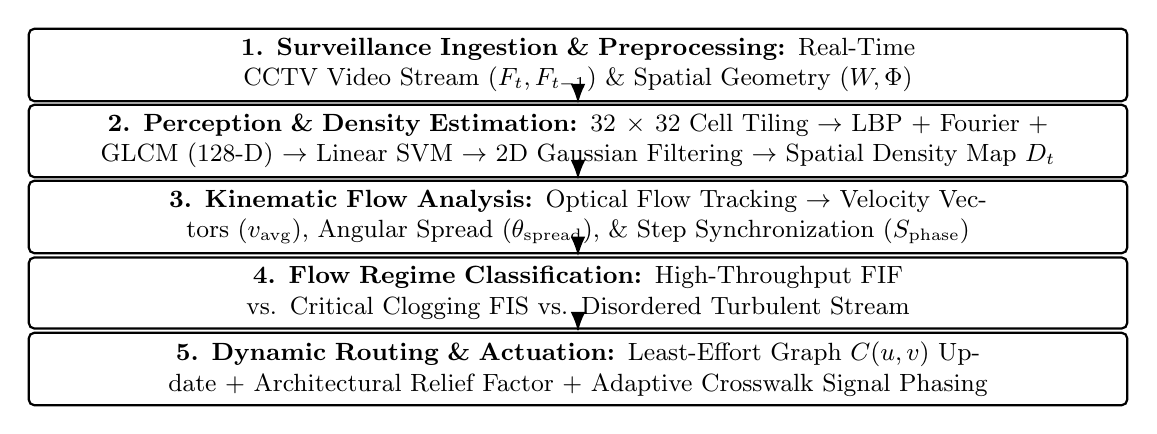
\begin{tikzpicture}[
    node distance=0.38in,
    auto,
    block/.style={
        rectangle,
        draw=black,
        fill=white,
        thick,
        text width=5.4in,
        align=center,
        rounded corners=2pt,
        font=\small
    },
    line/.style={draw=black, -{Latex[length=2.5mm]}, thick}
]
    \node [block] (input) {\textbf{1. Surveillance Ingestion \& Preprocessing:} Real-Time CCTV Video Stream ($F_t, F_{t-1}$) \& Spatial Geometry ($W, \Phi$)};
    \node [block, below of=input] (cv) {\textbf{2. Perception \& Density Estimation:} $32\times 32$ Cell Tiling $\to$ LBP + Fourier + GLCM (128-D) $\to$ Linear SVM $\to$ 2D Gaussian Filtering $\to$ Spatial Density Map $D_t$};
    \node [block, below of=cv] (flow) {\textbf{3. Kinematic Flow Analysis:} Optical Flow Tracking $\to$ Velocity Vectors ($v_{\text{avg}}$), Angular Spread ($\theta_{\text{spread}}$), \& Step Synchronization ($S_{\text{phase}}$)};
    \node [block, below of=flow] (state) {\textbf{4. Flow Regime Classification:} High-Throughput FIF vs. Critical Clogging FIS vs. Disordered Turbulent Stream};
    \node [block, below of=state] (routing) {\textbf{5. Dynamic Routing \& Actuation:} Least-Effort Graph $C(u, v)$ Update + Architectural Relief Factor + Adaptive Crosswalk Signal Phasing};

    \path [line] (input) -- (cv);
    \path [line] (cv) -- (flow);
    \path [line] (flow) -- (state);
    \path [line] (state) -- (routing);
\end{tikzpicture}
\caption{Proposed End-to-End System Implementation Architecture and Workflow Diagram}
\label{fig:workflow}
\end{figure}

\subsection{Proposed System Architecture}
The system architecture integrates four cooperative modules:
\begin{itemize}
    \item \textbf{Module 1: Perception \& Density Mapping:} Extracts 128-D texture descriptors (LBP, Fourier, GLCM) from $32 \times 32$ cells, using a Linear SVM and Gaussian smoothing to yield a continuous 2D density map ($D_t$) \cite{basalamah2020pedestrian, khan2026deep}.
    \item \textbf{Module 2: Flow \& Hazard Classifier:} Evaluates velocity ($\vec{V}$), $13^\circ$ angular spread ($\theta_{\text{spread}}$) \cite{bacik2023lane, bacik2025logic}, foot-sway synchronization ($S_{\text{phase}}$) \cite{scienceadv2025foot}, and intrusion index ($I_{\text{num}}$) to triage flow into Normal, FIF, Disordered, or FIS regimes.
    \item \textbf{Module 3: Least-Effort Evacuation Routing:} Models layout as a directed graph $G(V,E)$ via Least-Effort principles \cite{zipf1949human, guy2010pledestrians}, computing dynamic edge costs with merge and bottleneck penalties to bypass clogged nodes.
    \item \textbf{Module 4: Signal Actuation \& Alerting:} Computes real-time crosswalk walk-phase extensions ($S_{\text{adjust}} = \min(15.0, D_t \times 2.5)$ s) \cite{maitra2024kolkata} and distributes emergency alerts via MQTT.
\end{itemize}

\subsection{Implementation Roadmap and Phased Work Plan}
The work plan spans four sequential phases over an 8-month timeline:
\begin{enumerate}
    \item \textbf{Phase I: Perception Pipeline (Months 1--2):} Dataset curation (UCF CC 50, CrowdHuman), feature extraction, and Linear SVM density training.
    \item \textbf{Phase II: Flow Kinematics \& Hazard Triage (Months 3--4):} Optical flow tracking, $13^\circ$ spread analysis, foot-sway detection, and FIS/FIF classification.
    \item \textbf{Phase III: Routing \& Actuation (Months 5--6):} Least-effort graph formulation, merge-penalty impedance modeling, and adaptive signal timing.
    \item \textbf{Phase IV: Integration \& Validation (Months 7--8):} System benchmarking, edge optimization ($\ge 25\text{ FPS}$), and dashboard deployment.
\end{enumerate}

\begin{table}[htbp]
\centering
\caption{Project Milestone and Implementation Work Plan}
\label{tab:work_plan}
\fontsize{10pt}{12pt}\selectfont
\begin{tabular}{@{}llp{3.1in}@{}}
\toprule
\textbf{Phase / Period} & \textbf{Target Module} & \textbf{Key Deliverables and Implementation Objectives} \\ \midrule
Phase I (M1--M2) & Perception Pipeline & Feature extraction engine, trained SVM classifier, spatial density maps ($D_t$). \\
Phase II (M3--M4) & Kinematic Flow Engine & Angular spread analyzer ($\theta_{\text{spread}}$), footstep sync metric, FIS/FIF hazard classifier. \\
Phase III (M5--M6) & Routing \& Signal Actuation & Merge-aware dynamic graph router, least-effort impedance solver, adaptive signal manager. \\
Phase IV (M7--M8) & Integration \& Deployment & Edge-optimized pipeline, IoT alert dashboard, latency benchmark ($\ge 25\text{ FPS}$). \\ \bottomrule
\end{tabular}
\end{table}

\section{Facilities Required for Proposed Work}
\begin{itemize}
    \item \textbf{Hardware Infrastructure:} Multi-core 64-bit workstation (Intel i7/Ryzen 7, $\ge 16\text{ GB}$ RAM), CUDA-capable NVIDIA GPU ($\ge 6\text{ GB}$ VRAM, compute capability $\ge 7.5$), and an edge deployment module (e.g., NVIDIA Jetson).
    \item \textbf{Software \& Tooling:} Linux/Windows OS, Python 3.10+, OpenCV (optical flow, texture extraction), Scikit-Learn (Linear SVM), PyTorch, NetworkX (graph modeling), MQTT broker, and Git for version control.
    \item \textbf{Datasets \& Test Feeds:} UCF CC 50 \cite{basalamah2020pedestrian}, CrowdHuman \cite{shao2018crowdhuman}, pedestrian safety survey data \cite{maitra2024kolkata}, and real-world CCTV crosswalk feeds.
\end{itemize}

% =========================================================================
% 5. REFERENCES (Chronological Order, 18 Authentic References)
% =========================================================================
\begin{thebibliography}{99}
\fontsize{10pt}{12pt}\selectfont

\bibitem{zipf1949human}
G.~K. Zipf, \emph{Human Behavior and the Principle of Least Effort: An Introduction to Human Ecology}, Addison-Wesley Press, Cambridge, MA, USA, 1949.

\bibitem{helbing1995social}
D.~Helbing and P.~Molnar, ``Social force model for pedestrian dynamics,'' \emph{Physical Review E}, vol.~51, no.~5, pp. 4282--4286, 1995.

\bibitem{helbing2000simulating}
D.~Helbing, I.~Farkas, and T.~Vicsek, ``Simulating dynamical features of escape panic,'' \emph{Nature}, vol. 407, no. 6803, pp. 487--490, 2000.

\bibitem{guy2010pledestrians}
S.~J. Guy, J.~Chhugani, S.~Curtis, P.~Dubey, M.~Lin, and D.~Manocha, ``PLEdestrians: A least-effort approach to crowd simulation,'' in \emph{ACM SIGGRAPH/Eurographics Symposium on Computer Animation}, Madrid, Spain, 2010, pp. 119--128. \url{http://gamma.cs.unc.edu/PLEdestrians/}

\bibitem{depta2014self}
F.~Depta, L.~Liu, and N.~A. Suleman, ``Self-organized pedestrian crowd dynamics: An applet simulating intersecting pedestrian streams,'' Institute for Theoretical Physics, Goethe University Frankfurt, Tech. Rep., 2014.

\bibitem{liao2017faster}
W.~Liao, A.~Seyfried, J.~Zhang, M.~Boltes, X.~Zheng, and Y.~Zhao, ``Pedestrian crowd dynamics in merging sections: Revisiting the `faster-is-slower' phenomenon,'' \emph{Physica A: Statistical Mechanics and its Applications}, vol. 487, pp. 211--222, 2017.

\bibitem{shao2018crowdhuman}
S.~Shao, Z.~Zhao, B.~Li, T.~Xiao, G.~Yu, X.~Zhang, and J.~Sun, ``CrowdHuman: A benchmark for detecting human in a crowd,'' \emph{arXiv preprint arXiv:1805.00123}, 2018.

\bibitem{basalamah2020pedestrian}
S.~Basalamah and S.~D. Khan, ``Pedestrian crowd detection and segmentation using multi-source feature descriptors,'' \emph{International Journal of Advanced Computer Science and Applications}, vol.~11, no.~1, pp. 581--588, 2020.

\bibitem{corbetta2021physics}
A.~Corbetta and F.~Toschi, ``Physics of collaborative and non-collaborative pedestrian flow,'' \emph{Annual Review of Condensed Matter Physics}, vol.~12, pp. 325--346, 2021.

\bibitem{martinez2022computer}
S.~Mart{\'\i}nez-D{\'\i}az, I.~P{\'e}rez, and F.~G. Benitez, ``Crowd safety and pedestrian traffic: Applications of artificial intelligence, computer vision, physics and econometric methods,'' \emph{Transportation Research Part C: Emerging Technologies}, vol. 140, p. 103708, 2022.

\bibitem{bacik2023lane}
K.~A. Bacik, G.~Sobota, B.~Bacik, and T.~Rogers, ``Lane formation in bidirectional pedestrian flow: An imbalance in turning maneuvers,'' \emph{Physical Review Research}, vol.~5, no.~3, p. 033105, 2023.

\bibitem{morth2023report}
Ministry of Road Transport and Highways, ``Road accidents in India 2022,'' Transport Research Wing, MoRTH, Government of India, New Delhi, Tech. Rep., 2023.

\bibitem{maitra2024kolkata}
B.~Maitra, ``Kolkata’s road-safety push must begin with pedestrians: Analysis of pedestrian fatalities and infrastructure risk in West Bengal,'' Department of Civil Engineering, IIT Kharagpur, Report, 2024.

\bibitem{bacik2025logic}
K.~A. Bacik, G.~Sobota, B.~Bacik, and T.~Rogers, ``Fluid-dynamic model of pedestrian lane formation and the transition to angular disorder,'' \emph{Proceedings of the National Academy of Sciences}, vol. 122, no.~12, p. e2418301122, 2025.

\bibitem{scienceadv2025foot}
Y.~Wang, D.~Chen, and H.~Zhang, ``Bottom-up foot-tracking reveals spontaneous movement synchronization at the onset of crowd jamming,'' \emph{Science Advances}, vol.~11, no.~8, p. eadw2688, 2025.

\bibitem{mai2025evaluating}
W.~Mai, D.~Duives, P.~Krishnakumari, and S.~Hoogendoorn, ``Evaluating crowd flow forecasting algorithms for indoor pedestrian spaces: A benchmark using a synthetic dataset,'' \emph{IEEE Transactions on Intelligent Transportation Systems}, vol.~26, no.~6, pp. 7953--7966, 2025.

\bibitem{khan2026deep}
S.~D. Khan, H.~Ullah, and M.~S. Basalamah, ``Deep spatio-temporal density regression for real-time crowd choke point prevention in transit terminals,'' \emph{IEEE Transactions on Intelligent Transportation Systems}, vol.~27, no.~2, pp. 1104--1118, 2026.

\end{thebibliography}

\end{document}
